\chapter{Implementatie}
\label{chap:implementatie}
Om de hypothesen (\sectionref{sec:onderzoeksvraag}) af te toetsen, moet er een werkende implementatie zijn van GeoSPARQL. De structuur van dit hoofdstuk zal dezelfde volgorde aannemen als hoe de implementatie is verlopen. Dit toont een zekere structuur, zodat elk deel steeds onmiddellijk getest kan worden. 


\section{Comunica}
\label{sec:impl_comunica}
Zoals eerder aangehaald speelt Comunica een zeer belangrijke rol bij deze implementatie van GeoSPARQL (zie \sectionref{sec:comunica}). Hierbij (dankzij de modulariteit) is het mogelijk om een actor aan te maken voor het afhandelen van GeoSPARQL-functionaliteiten. Deze actor maakt gebruik van ``sparqlalgebrajs'' om de SPARQL query om te vormen naar SPARQL algebra en van ``sparqlee'' om deze SPARQL algebra correct uit te werken. 

\subsection{Sparqlalgebrajs}
\begin{listing}[ht]
    \begin{minted}{sparql}
        SELECT ?f
        WHERE {
            my:A my:hasExactGeometry ?aGeom .
            ?aGeom geo:asWKT ?aWKT .
            ?f my:hasExactGeometry ?fGeom .
            ?fGeom geo:asWKT ?fWKT .
            FILTER (geof:sfContains(?aWKT, ?fWKT) && !sameTerm(?aWKT, ?fWKT))
        }
    \end{minted}
    \caption{Example SPARQL query.}
    \label{listing:sparqlalgebrajs_query}
\end{listing}

\begin{listing}[ht]
    \begin{minted}{json}
        {
        ...,
        expression: {
            type: 'expression',
            expressionType: 'operator',
            operator: '&&',
            args: [
            {
                type: 'expression',
                expressionType: 'named',
                name: NamedNode {
                id: 'http://www.opengis.net/def/function/geosparql/sfContains'
                },
                args: [
                {
                    type: 'expression',
                    expressionType: 'term',
                    term: Variable { id: '?aWKT' }
                },
                {
                    type: 'expression',
                    expressionType: 'term',
                    term: Variable { id: '?fWKT' }
                }
                ]
            },
            {
                type: 'expression',
                expressionType: 'operator',
                operator: '!',
                args: [
                {
                    type: 'expression',
                    expressionType: 'operator',
                    operator: 'sameterm',
                    args: [
                    {
                        type: 'expression',
                        expressionType: 'term',
                        term: Variable { id: '?aWKT' }
                    },
                    {
                        type: 'expression',
                        expressionType: 'term',
                        term: Variable { id: '?fWKT' }
                    }
                    ]
                }
                ]
            }
            ]
        }
        }
    \end{minted}
    \caption{Example SPARQL algebra.}
    \label{listing:sparqlalgebrajs_algebra}
\end{listing}

Sparqlalgebrajs zorgt er onder andere voor dat de filter omgezet wordt naar een boomstructuur die recursief kan worden doorlopen. Deze omvorming is te zien in \listingref{listing:sparqlalgebrajs_query} en \listingref{listing:sparqlalgebrajs_algebra}. In \listingref{listing:sparqlalgebrajs_query} is een voorbeeld van een correct GeoSPARQL query te zien (ter informatie: deze query haalt alle vormen in die geografisch in ``my:A'' liggen, maar niet ``my:A'' zelf zijn), maar voor het uitvoeren van deze query moet deze eerst omgevormd worden naar SPARQL algebra. Vanwege de grootte van het resultaat is slechts de essentie hiervan terug te vinden in \listingref{listing:sparqlalgebrajs_algebra}. Aangezien het gaat over de filterfunctie, is enkel dat deel terug te vinden. Hierbij is zeer duidelijk de recursieve boomstructuur te vinden, waarbij in de wortel van de boom de operator ``\&\&'' te zien is. Dit blad in de boom zal vervolgens een linker- en rechterkind hebben. Deze zijn te vinden in het veld ``args'' en krijgen de waarde van opnieuw de uitkomst van twee bladeren. Ditmaal zijnde de ``sfContains'' functie aan de linker helft en de ``!'' operator aan de rechter helft. Dit wordt op deze manier recursief uitgevoerd.

\subsection{Sparqlee}
Sparqlee is een SPARQL \textit{expression evaluator}. Dit betekent dat sparqlee een SPARQL algebra expressie zal evalueren. Sparqlee is bij deze implementatie gebruikt voor het maken van de GeoSPARQL functionaliteiten, omdat sparqlee zelf als de recursieve boomstructuur van sparqlalgebrajs volledig afhandelt voor SPARQL queries. Dit is belangrijk voor de belangrijkste vereiste voor GeoSPARQL, namelijk het hebben van een werkende SPARQL implementatie. Zo zal sparqlee eerst de volledige expressie controleren om te zien of het geheel verwerkt kan worden. Dit is dus enkel het geval als sparqlee de verschillende functies en operators correct kan afhandelen. In dit specifieke geval betekent het dus dat sparqlee de GeoSPARQL functies moet kunnen uitvoeren. Hiervoor is dezelfde programmeerstijl gehanteerd als deze die al aanwezig is in sparqlee zelf.

\subsection{Verbeteringen}
Een eerste verbetering aan deze eerste keuze is meteen dat deze GeoSPARQL functies niet in sparqlee gemaakt zouden mogen worden. Sparqlee is louter een SPARQL \textit{expression evaluator}, wat betekent dat deze niet meer dan enkel SPARQL hoort te ondersteunen. De oplossing hiervoor is het ondersteunen van \textit{custom functions} binnen sparqlee (dit staat bovendien binnen de specificaties van SPARQL). Indien deze \textit{custom functions} ondersteund zouden worden binnen sparqlee, dan zou het mogelijk zijn om de functies te implementeren binnen de hiervoor gemaakte actor in Comunica. Op deze manier kan deze dan geïnjecteerd worden in sparqlee. Het implementeren van deze \textit{custom functions} functionaliteit binnen sparqlee is echter te complex en tijdrovend voor de eerder kleine impact op deze masterproef. Dit blijft echter wel een vereiste voor de modulariteit, maar dit wordt gezien als \textit{future work}. 
\newpage
\section{Datastructuur}
\label{sec:datastructuur}
Voordat begonnen kan worden aan de effectieve oplossing van GeoSPARQL functies, moet de gepaste datastructuur gekozen worden om dit te kunnen realiseren. Zoals beschreven in \sectionref{subsec:geosparql_architecture}, moet er ondersteuning zijn voor zowel ``Geometry'' als ``Feature'' objecten. 

\subsection{GeoJSON}
Om dit te kunnen ondersteunen is er gekozen voor een vaker gebruikt formaat, genaamd GeoJSON. GeoJSON biedt ondersteuning voor zowel ``Geometry'' als ``Feature'' objecten, waarbij ``Feature'' objecten een ``Geometry'' object bevatten, naast andere attributen. Bovendien ondersteunt GeoJSON de volgende vormen: ``Point'', ``LineString'', ``Polygon'', ``MultiPoint'', ``MultiLineString'' en ``MultiPolygon''. Op deze manier zijn alle voorwaarden van de architectuur voor GeoSPARQL voldaan. Het volgende probleem is dan: hoe kan een WKT string omgevormd worden naar GeoSPARQL?

\subsection{Terraformer}
Terraformer is een geografische toolkit voor het werken met onder andere geometrieën, geografie en formaten. Verder is Terraformer opgesplitst in enkele modules. Hier wordt verder (zie \sectionref{sec:topologische_functies}) op terug gekomen. Voorlopig wordt enkel verder ingegaan op de Terraformer WKT parser. Deze module is gemaakt om te voorzien in een eenvoudige omzetting van WKT string naar GeoJSON en indien gewenst ook in de omgekeerde richting. Op deze manier kan een geserialiseerde vorm (namelijk WKT string) omgezet worden naar GeoJSON, zodat nu verder gegaan kan worden met de implementatie. 



 
\newpage
\section{Topologische functies}
\label{sec:topologische_functies}
Een van de belangrijkste functionaliteiten van GeoSPARQL is het topologisch van elkaar kunnen onderscheiden van vormen. Hiervoor zijn er drie verschillende relatiefamilies (zoals eerder aangehaald, zie \subsectionref{subsec:topologische_relaties}). Vanwege de eerder korte periode voor deze masterproef is ervoor gekozen om de focus te leggen op slechts één van deze families, namelijk de ``Simple Features'' familie. Om niet te vaak in herhaling te vallen kan best terugverwezen worden naar \subsubsectionref{subsubsec:simple_features} om te kijken naar de specificaties van deze familie. Om de eerste functie te maken is gekozen voor de ``sfContains'' functie. De \textit{contains}-functie is een veel gebruikte en voor de hand liggende functie, die gaat controleren of een vorm binnen een andere vorm ligt. Om de verschillende functies te testen werd een eenvoudige testset gecreëerd. Deze testset is te zien in \figureref{fig:illustration_spatial_data}. Om tot een eerste uitkomst te komen, was er al een zeer goede oplossing. Dit bleek Terraformer te zijn.

\begin{figure}[ht]
    \centering
    
\includegraphics[width=0.5\linewidth]{images/geosparql_example.png}
    \caption{Illustratie geospatiale data van \cite{ogcdocs}}
    \label{fig:illustration_spatial_data}
\end{figure}

\subsection{Terraformer}
Terraformer was een eerste en zeer voor de hand liggende keuze, omdat deze reeds gebruikt werd voor de omzetting van WKT naar GeoJSON. Zo heeft Terraformer een module voor het werken met GeoJSON. De module heet Terraformer Core. Deze module voorziet functies voor onder andere het controleren of een vorm binnen een andere vorm ligt en om te controleren of een vorm een andere vorm snijdt. Dit is welliswaar te beperkt om de volledige ``Simple Features'' familie te implementeren, maar voor de ``sfContains'' en nadien voor zowel de ``sfIntersects'' en de ``sfDisjoint'' functies is dit zeker een goed begin. 

Na het maken van de implementatie, bleken er toch enkele problemen te zijn met de ``contains'' functie van Terraformer. Zo valt onmiddellijk op dat er vele randgevallen zijn die niet correct werken. Enkele voorbeelden daarvan zijn de volgende:
\begin{itemize}
    \item Polygoon ``contains'' lijn: wanneer de lijn van een hoekpunt naar een ander hoekpunt gaat (dus wanneer het een zijde of een diagonaal is), zou dit ``true'' moeten geven, maar dit geeft ``false''.
    \item Polygoon ``contains'' polygoon: wanneer de polygonen een hoekpunt delen (dus deze ligt erin, maar ligt helemaal in de hoek), zou dit ``true'' moeten geven, maar dit geeft ``false''.
\end{itemize}

Om, gebruik makend van Terraformer, deze problemen op te lossen zou teveel code aangepast moeten worden. Aangezien deze randgevallen zeer vaak voorkomen (en aangezien de kans reëel is dat er nog meerdere andere fouten zijn), werd besloten om een andere oplossing te zoeken die meer bruikbaar is voor het geheel, zoals de andere topologische functies.

\subsection{Manueel}
Het eerstvolgende idee was om dit manueel op te lossen. Dit leek een logische oplossing, omdat zo alle functies met zekerheid gemaakt kunnen worden en dit met een implementatie die conform is met de OGC-standaarden. Hier werd echter vrij snel van afgeweken vanwege de complexiteit. Het uitgevoerde onderzoek wordt hieronder beschreven, opnieuw voor het voorbeeld van de ``contains'' functie. Hierbij werd ook enkel aandacht gegeven aan de enkelvoudige vormen (dus ``Point'', ``LineString'' en ``Polygon''). De gedachtengang hierbij was dat de meervoudige vorm identiek was, maar zich meerdere keren herhaalt.

\subsubsection{Point}
Bij het beginnen van een eigen implementatie is het eenvoudigste om te beginnen bij een punt. Hierbij is het namelijk zo dat een punt enkel in een punt ligt wanneer dit punt exact hetzelfde is. Het controleren of een lijn of een polygoon in een punt ligt is nog eenvoudiger, dit is namelijk niet mogelijk (en bijgevolg dus altijd ``false'').  

\subsubsection{LineString}
Het volgende deel is logischerwijs controleren wat binnen een lijn kan liggen. Voor een punt is dit wiskundig eenvoudig op te lossen, door voor elk deel van de lijn de richtingscoëfficient uit te rekenen en vervolgens te kijken of het punt op de lijn ligt. Hierbij moet wel opgelet worden, aangezien het deel van de lijn niet oneindig doorloopt. Dit is evenwel eenvoudig op te lossen door te controleren dat de x-coördinaat van het punt tussen de x-coördinaten van de uiteinden van de lijn ligt.

Bij het controleren of een lijn in een andere lijn ligt, kan dezelfde techniek als bij een punt gebruikt worden. Hierbij moet voor elk deel van de mogelijks binnen liggende lijn gecontroleerd worden of de uiteinden op de eerste lijn liggen. Ook moet er gecontroleerd worden of de richtingscoëfficient van beide lijnen in dit deel (het volledige deel) identiek is. Indien deze voorwaarden voldaan zijn, dan ligt de lijn binnen de andere lijn. 

De controle of een polygoon binnen een lijn ligt is overbodig. Dit is namelijk onmogelijk, bijgevolg kan deze functie rechtstreeks ``false'' als uitkomst geven.

\subsubsection{Polygon}
Het laatste en moeilijkste deel is controleren of een vorm binnen een polygoon ligt. Het eerste deel is het controleren of een punt binnen een polygoon ligt. Intuïtief wordt direct gedacht aan het wiskundig beschrijven van een vlak, maar dit is echter niet bruikbaar. Vervolgens kan gecontroleerd worden of het punt onder of boven een lijn ligt, om zo te proberen achterhalen of dit betekent dat het punt binnen de polygoon ligt. Het probleem heeft echter een eenvoudigere oplossing dan dit. Wanneer het punt op een lijn van de polygoon ligt, is meteen geweten dat de ``contains'' functie ``true'' moet weergeven. Wanneer dit niet het geval is, kan een andere techniek gebruikt worden. Zo kan een horizontale lijn getrokken worden, vertrekkend vanuit het punt en helemaal naar rechts (met oneindige lengte). Wanneer nu geteld wordt met hoeveel lijnen van de polygoon deze lijn kruist, is de uitkomst gekend. Het punt ligt namelijk binnen de polygoon wanneer het aantal kruissende lijnen een oneven aantal is. Deze techniek is geïllustreerd in \figureref{fig:polygon_contains_point}.

\begin{figure}
    \centering
    
\includegraphics[width=0.5\linewidth]{images/polygon_contains_point.png}
    \caption{Voorbeeld polygon contains point.}
    \label{fig:polygon_contains_point}
\end{figure}

Het volgende deel is het controleren of een lijn binnen een polygoon ligt. Hiervoor is er opnieuw een techniek. Voor de lijn moet gecontroleerd worden of een punt binnen de polygoon ligt. Indien dit het geval is, moet ook nog eens gecontroleerd worden of de lijn snijdt met een rand van de polygoon. Dit betekent dat elke lijn van de rand van de polygoon gecontroleerd moet worden. Het controleren of lijnen snijden is opnieuw wiskundig aan te pakken, maar hier wordt niet verder op ingegaan. Deze techniek is geïllustreerd in \figureref{fig:polygon_contains_line}.

\begin{figure}
    \centering
    
\includegraphics[width=0.3\linewidth]{images/polygon_contains_line.png}
    \caption{Voorbeeld van polygon contains line.}
    \label{fig:polygon_contains_line}
\end{figure}

Het laatste deel hierbij is het controleren of een polygoon binnen een polygoon ligt. Hiervoor zou intuïtief gedacht kunnen worden aan het controleren of alle punten van de (vermoedelijk) binnenste polygoon binnen de andere polygoon liggen. Zoals geïllustreerd in \figureref{fig:polygon_contains_polygon} is dit niet altijd het geval. Dit is enkel mogelijk indien de buitenste vorm convex (= bolvormig) is. Aangezien dit in vele gevallen niet zo is, zou het verlies van performantie zijn om hierop te controleren. Een correcte techniek is echter controleren of één enkel punt van de (vermoedelijk) binnenste polygoon binnen de andere polygoon ligt. Vervolgens volstaat het om te controleren of er een lijn van de rand van de ene polygoon snijdt met een lijn van de rand van de andere polygoon. Indien er snijdende lijnen zijn, zal de ``contains'' functie ``false'' teruggeven. Hierbij wordt ook duidelijk dat deze berekeningen computationeel intensief worden, zeker in het geval van queryen. Dit kan nog verbeterd worden door de lijnintersectietests te versnellen met het ``\textit{sweep line}'' algoritme, maar hier wordt niet verder op ingegaan. In het voorbeeld in \figureref{fig:polygon_contains_polygon} is de gekleurde polygoon diegene die getest wordt om binnen de andere te liggen.

\begin{figure}
    \centering
    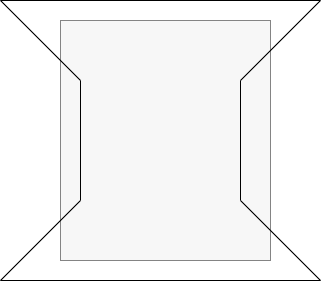
\includegraphics[width=0.3\linewidth]{images/polygon_contains_polygon.png}
    \caption{Voorbeeld van polygon contains polygon.}
    \label{fig:polygon_contains_polygon}
\end{figure}


\subsubsection{Extra moeilijkheden}
De eerder vernoemde technieken zijn al vrij ingewikkeld en dit is slechts voor de ``contains'' functie. Hier zouden nog meerdere andere technieken gebruikt moeten worden om de andere functies te implementeren. Dit wordt nog ingewikkelder wanneer ook rekening gehouden wordt met de veelvoudige vormen zoals ``MultiPoint'', ``MultiLineString'' en ``MultiPolygon''. Hierbovenop is er ook nog geen rekening gehouden met de binnenste ring van de polygonen, die een deel van het vlak excluderen. Dit is nog een extra moeilijkheidsfactor waar rekening mee moet worden gehouden.  

Zo zijn er vele nadelen aan het zelf implementeren hiervan. Een eigen implementatie bevat snel fouten bij de vereiste functionaliteiten zoals ze hierboven beschreven werden. Ook moet dit uitvoerig getest worden, wat best door een maximaal aantal gebruikers gebeurt. Bovendien moeten de meest performante algoritmes gebruikt worden, zodat dit bruikbaar is voor queries. Al deze redenen verwerpen het zelf implementeren. Daarom werd ervoor gekozen om overgegaan ``Turf.js'' te gebruiken.

\subsection{Turf.js}
``Turf.js'' is een modulaire geospatiale engine die gemaakt is in JavaScript. Zo is Turf een JavaScript \textit{library} die werkt aan de hand van GeoJSON. Het is een verzameling van kleine modules, zodat gebruik kan gemaakt worden van exact wat nodig is voor de \textit{use case}. Turf gebruikt naar eigen zeggen de nieuwste algoritmes, wat een pluspunt is voor de performantie. Bovendien heeft Turf een uitgebreide \textit{community}, wat ervoor zorgt dat mogelijke fouten in de implementatie gevonden en opgelost worden. Zo kan een bug opgelost worden door de nieuwste versie binnen te halen.

Turf voorziet vele methoden om te gebruiken in eigen berekeningen. Daarnaast heeft Turf al enkele \textit{build in} functies, zoals ``booleanContains'', ``booleanDisjoint'' en ``booleanOverlap''. Deze functies zijn exact wat nodig is. Een overzicht van de functies die gebruikt zijn voor de implementatie van de ``Simple Features'' familie is te zien in \tableref{tab:turf_functions}.

\begin{table}[ht]
    \centering
    \begin{tabular}{ |p{2cm}|p{2cm}|p{8cm}| } 
        \hline
        \rowcolor{TableHeaderColor} GeoSPARQL functie & Turf.js functie & Opmerkingen \\ \hline
        
        \rowcolor{TableColor} sfEquals & booleanEqual & De functie van Turf is volledig conform met de documentatie. \\ \hline

        \rowcolor{TableColor} sfDisjoint & booleanDisjoint & De functie van Turf blijkt volledig conform te zijn met de documentatie van GeoSPARQL. Deze bevat echter een bug waarbij twee evenwijdige en overlappende lijnen toch ``disjoint'' zouden zijn. \\ \hline

        \rowcolor{TableColor} sfIntersects & !booleanDisjoint & Deze functie heeft hetzelfde probleem als sfDisjoint, aangezien deze het inverse is. \\ \hline

        \rowcolor{TableColor} sfTouches & / & Turf heeft nog geen functie die gebruikt kan worden voor deze functionaliteit. \\ \hline

        \rowcolor{TableColor} sfWithin & booleanWithin & De functie van Turf blijkt volledig conform te zijn met de documentatie van GeoSPARQL. Deze bevat echter een bug bij het gebruik van de binnenste ring. \\ \hline

        \rowcolor{TableColor} sfContains & booleanContains & De functie van Turf blijkt volledig conform te zijn met de documentatie van GeoSPARQL. Deze bevat echter een bug bij het gebruik van de binnenste ring. \\ \hline

        \rowcolor{TableColor} sfOverlaps & booleanOverlap & De functie van Turf is niet volledig conform met de documentatie van GeoSPARQL. Het verschil hierbij is dat het voor Turf voldoende is om enkel de borders te laten overlappen, terwijl GeoSPARQL benadrukt dat ook de interiors moeten overlappen. \\ \hline

        \rowcolor{TableColor} sfCrosses & booleanCrosses & De functie ``booleanCrosses'' van Turf zou overeen moeten komen, maar deze heeft andere specificaties waardoor deze niet bruikbaar is.  \\ \hline
    \end{tabular}
    \caption{Implementatie GeoSPARQL functies (Simple Features familie) met ``Turf.js''.}
    \label{tab:turf_functions}
\end{table} 
\newpage
\section{Niet-topologische functies}
\label{sec:niet_topologische_functies}
De niet-topologische functies binnen GeoSPARQL zijn beperkter in hoeveelheid, ten opzichte van de topologische functies. In de plaats van het onderscheiden van vormen zorgen deze functies voor het uitvoeren van berekeningen. Dit kan bijvoorbeeld het opzoeken van de kortste afstand tussen twee vormen zijn of het samenvoegen van twee vormen om vervolgens een topologische functie erop los te laten. Aan deze functies wordt iets minder aandacht besteed dan aan de topologische functies omdat deze duidelijk minder gebruikt zullen worden. Toch is er een implementatie gemaakt voor de ``union'' en ``intersection'' functies. De ``union'' functie zal twee vormen samenvoegen tot één nieuwe vorm. De ``intersection'' functie zal dan weer kijken naar het deel dat twee vormen gemeenschappelijk hebben en dit terug geven. 

Voor het maken van deze implementaties is opnieuw gebruik gemaakt van Turf en dankzij de implementatie van sparqlee, die excellent gebruik maakt van het \textit{divide-and-conquer} (= verdeel en heers) programmeer principe, is deze implementatie op bijna identiek dezelfde manier als de topologische functies mogelijk.

\subsection{Beperkingen}
Aangezien gebruik gemaakt wordt van Turf, moet de manier van Turf gevolgd worden. Hierbij is het enkel mogelijk om de unie of intersectie te berekenen van polygonen. GeoSPARQL beschrijft echter dat deze functies beiden een geometrisch object terug moeten geven die alle punten representeert van het resultaat van deze functies. Dit impliceert dat het ook mogelijk moet zijn om deze functies toe te passen op punten en lijnen. Dit zou zelfs mogelijk moeten zijn om de combinatie van punten, lijnen en polygonen.

\begin{figure}
    \centering
    \begin{subfigure}[t]{0.5\linewidth}
        \centering
        
\includegraphics[width=0.3\linewidth]{images/union_example1.png}
        \caption{Voor union.}
        \label{fig:union_example1}
    \end{subfigure}%
    ~ 
    \begin{subfigure}[t]{0.5\linewidth}
        \centering
        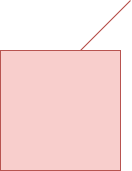
\includegraphics[width=0.3\linewidth]{images/union_example2.png}
        \caption{Resultaat union.}
        \label{fig:union_example2}
    \end{subfigure}
    \caption{Problematiek union.}
\end{figure}

Dit laatste is echter niet mogelijk met de huidige implementatie waar gebruik gemaakt wordt van ``Point'', ``MultiPoint'', ``LineString'', ``MultiLineString'', ``Polygon'' en ``MultiPolygon''. In \figureref{fig:union_example1} is een voorbeeld te zien van twee vormen waarvan de unie (= de vorm die alle punten van beide figuren samen bevat) genomen wordt. In \figureref{fig:union_example2} wordt dan weer aangetoond dat het resultaat van de unie van een ``LineString'' en een ``Polygon'' niet te representeren valt in één van de zes eerder genoemde vormen. Hiervoor zou gewerkt moeten worden met een soort ``GeometryColletion''. 
\newpage
\section{Referentiesysteem}
\label{sec:projecties}
Om een werkende implementatie te bekomen, is er nog een functionaliteit die ondersteund moet worden. Zo moet het mogelijk zijn om te werken met verschillende referentiesystemen. Om nog eens te benadrukken waarom dit belangrijk is, wordt dit geïllustreerd met een voorbeeld. Verschillende landen of zelfs delen van landen liggen op andere aardplaten die los van elkaar bewegen of zelfs tegen elkaar botsen. Hierdoor kunnen landen ten opzichte van elkaar bewegen. Het best voorbeeld hiervan is Australië dat jaarlijks wat kan verplaatsen. Op deze manier zou na enkele jaren elke geografische entiteit opnieuw vastgelegd moeten worden. Hiervoor wordt gebruik gemaakt van aparte referentiesystemen. Dit is een manier om een punt te beschrijven in coördinaten ten opzichte van een relatief punt. Om echter coördinaten in verschillende referentiesystemen te kunnen vergelijken met elkaar, moeten deze eerst omgerekend worden naar hetzelfde referentiesysteem.

Voor het oplossen van dit probleem bestaan twee mogelijkheden. Ofwel worden beide referentiesystemen omgerekend naar één op voorhand gedefinieerd referentiesysteem, ofwel wordt één van beide referentiesystemen naar de andere omgerekend. Er is gekozen voor de tweede optie om twee redenen. In dit geval moet voor elk koppel vormen, dat vergeleken wordt, slechts één vorm herrekend worden, wat zorgt voor een betere performantie. De tweede reden is dat het OGC zelf voorschrijft dat gewerkt moet worden in het referentiesysteem van de eerste vorm.

\subsection{Proj4js}
``Proj4js'' is een \textit{library} die zorgt voor het transformeren van coördinaten van het ene referentiesysteem naar coördinaten van het andere referentiesysteem. Hierbij zijn al enkele projecties op voorhand gedefinieerd binnen Proj4, maar het is ook mogelijk om zelf nieuwe projecties toe te voegen. Proj4 is dan ook de gebruikte \textit{library} voor het uitvoeren van deze berekening bij de gemaakte implementatie.

\subsection{Beperkingen}
Bij deze functionaliteit zijn er nog wel enkele beperkingen. Er zijn nog niet veel referentiesystemen beschreven binnen GeoSPARQL, waardoor het slechts in beperkte mate mogelijk is om van deze functionaliteit gebruik te maken. De architectuur van hoe hiermee gewerkt wordt, is echter wel in orde. Kortom betekent dit dat het nog niet zeer handig is om te gebruiken, maar dat het wel klaar is om in de toekomst toegepast te worden. 
\newpage
\section{Testomgeving}
\label{sec:testomgeving}
\todo{verwijzen hiernaar bij hypothesen}
In de voorgaande secties werd beschreven hoe de implementatie van GeoSPARQL gemaakt is. Nu er een werkende implementatie is, is het mogelijk om over te gaan naar de volgende stap. Hier zijn drie doelen bij, namelijk:
\begin{enumerate}
    \item Visualiseren van het geheel, met makkelijk aanpasbare queries.
    \item Omgeving voor het geven van demonstraties van de implementatie.
    \item Omgeving voor het uitvoeren van tests, voor het aftoetsen van de hypothesen.
\end{enumerate}

Om dit te bereiken is gebruik gemaakt van de ``jQuery Widget'' van Comunica. Deze geeft een grafische \textit{user interface}, die toestaat om te queryen over één of meerdere bronnen. Hierbij is het mogelijk om de bronnen zelf in te geven. Daarnaast is het ook mogelijk om de query zelf in te geven. Deze geeft een overzicht van het resultaat terug en geeft een ``execution log'' terug, zodat gecontroleerd kan worden welke stappen doorlopen werden voor het bekomen van het resultaat. Het geheel hiervan is zichtbaar in \figureref{fig:testomgeving}.

\begin{figure}
    \centering
    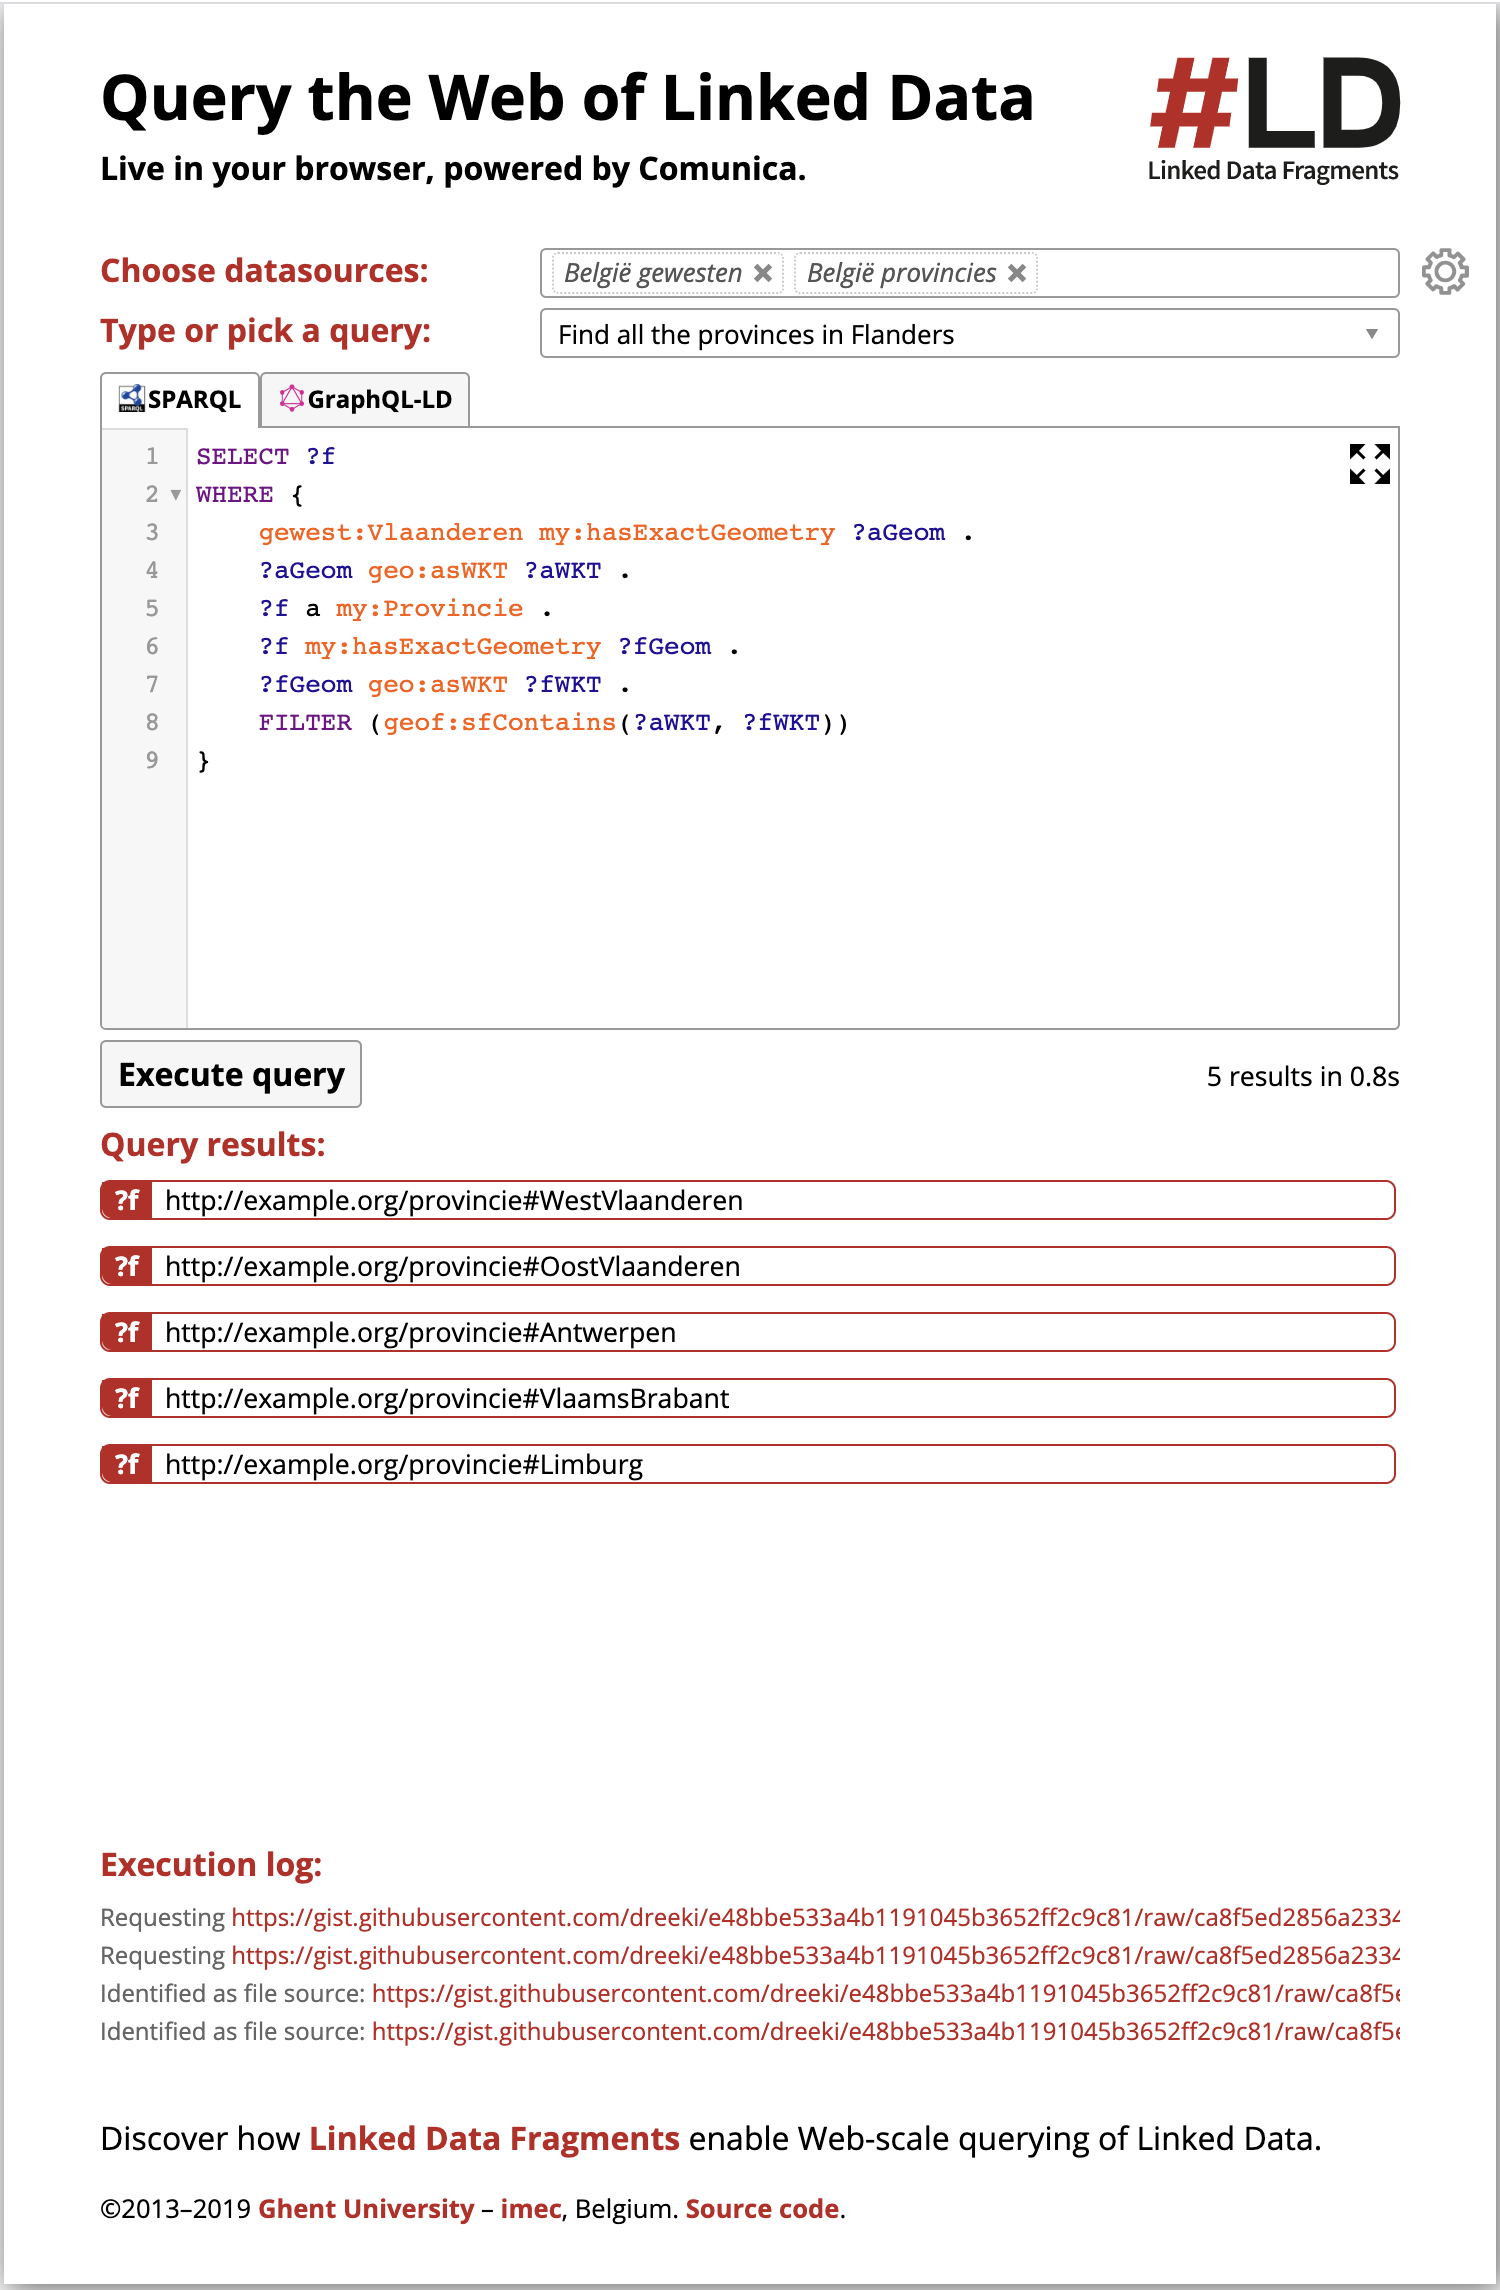
\includegraphics[width=0.8\linewidth]{images/testomgeving.png}
    \caption{Screenshot van online geplaatste testomgeving.}
    \label{fig:testomgeving}
\end{figure}

Hiermee is het eerste doel onmiddelijk bereikt. Dankzij het uitzicht dat zeer gelijkaardig is aan andere gekende \textit{query engines}, is dit zeer geschikt voor het geven van demonstraties. Ten slotte, zoals eerder vermeld, is het mogelijk om zowel de bronnen in te geven als de volgorde van uitvoering te bekijken. Hierdoor is het uitermate geschikt voor het uitvoeren van tests en voor het aftoetsen van de hypothesen. 
\newpage
\section{Overzicht}
\label{sec:impl_overzicht}
Om kort een overzicht te schetsen, zal deze sectie de implementatie overlopen en hierbij beschrijven wat gemaakt is en wat nog te doen is. Bij de vorige secties werden de functionaliteiten besproken in volgorde van implementatie. In dit overzicht zullen ze besproken worden in volgorde van uitwerking. Er kan alleszinds wel besloten worden dat een complete implementatie van GeoSPARQL zeer veel werk vraagt. In het kader van deze masterproef is hier al een deel van gemaakt, maar hier moet nog verder aan gewerkt worden.

\subsection{Huidige status}
Bij deze implementatie wordt eerst gecontroleerd of het gaat over een GeoSPARQL functionaliteit. Wanneer dit het geval is, zal eerst de linker- en rechterparameter recursief opgelost worden, zodat de functionaliteit effectief opgelost kan worden. Bij het oplossen van deze functionaliteit zal eerst de ``WKT string'' omgezet worden naar een GeoJSON object, waarbij gecontroleerd wordt of er een projectie (= referentiestelsel) meegegeven is (indien niet wordt gewerkt met de standaard waarde, genaamd ``WGS84''). Indien beide parameters van de functie niet dezelfde projectie zouden hebben, dan worden de coördinaten van de tweede parameter omgerekend naar de respectievelijke waarden van de projectie van de eerste parameter. Eenmaal dat dit gedaan is kan de functie eenvoudig uitgewerkt worden met behulp van ``Turf.js''. Dit resultaat wordt dan teruggegeven, zodat de boomstructuur dit kan gebruiken voor de verdere uitwerking van de recursieve structuur. Voor niet-topologische functies kan het nodig zijn om een GeoJSON object terug te geven. Om een uniforme werking van sparqlee te kunnen behouden, wordt dit GeoJSON object opnieuw geserialiseerd naar WKT formaat. 

\subsection{Toekomstwerk}
\label{subsec:toekomstwerk}
Aangezien deze implementatie slechts een beperkte implementatie van GeoSPARQL is, zal hier in de toekomst nog verder aan gewerkt moeten worden. Er wordt momenteel slechts in zeer beperkte mate ondersteuning aangeboden voor het gebruik van ``Feature''. Er is ook enkel ondersteuning voor ``WKT strings'' en niet voor het alternatieve ``GML'' formaat. Vervolgens moet er een aanvulling gemaakt worden van zowel de topologische functies als de niet-topologische functies. Bij de topologische functies is enkel gekeken naar de ``Simple Features'' familie (en deze is ook niet helemaal compleet), maar er zijn nog twee andere families. Bij de niet-topologische functies zijn er slechts twee functies geïmplementeerd, zijnde de ``union'' en de ``intersection'' functies. Hier zijn er nog verscheidene andere functies. Ten slotte moet het mogelijk zijn om deze functies te gebruiken in de vorm van predicaat. Hiervoor moet er een functionaliteit zijn voor het herschrijven van de queries. Deze is totaal niet gebruikt, maar is wel nodig voor een volledige implementatie van GeoSPARQL.  
\newpage